\section{MDA Framework} \label{sec:mda}
Hunicke et al. (2004) \cite{Hunicke2004} published their Mechanics-Dynamics-Aesthetics (MDA) framework as a formal approach towards establishing a clear understanding of games.
It aims to connect the fields of game design, development, criticism, and technical research.
Creating a common vocabulary allows to reason about game artifacts and iteratively improve them.

As videogames grow more and more complex it becomes increasingly difficult to keep track of all aspects shaping a game and influencing each other.
Small changes to one area might propagate through different structures and change gameplay in unexpected ways.
This emphasizes the need for an abstract, clear view on games as a coherent system.

The MDA framework (Figure \ref{fig:mda}) starts by breaking apart the consumption of games into: (1) Rules, (2) system, and (3) ``fun''.
It consequently translates these components into their design counterparts: (1) Mechanics, (2) dynamics, and (3) aesthetics.
Mechanics refer to the bare-bone data representations and algorithms at the heart of a game.
At run-time dynamics are produced by the underlying mechanics through player inputs and subsequent dynamic outputs.
Finally, the previous components results in aesthetics which describe the emotional responses of players.
This chain already indicates that changes to the basic mechanics will propagate through dynamics and emerge as different gameplay experiences.

\begin{figure}[H]
    \centering
    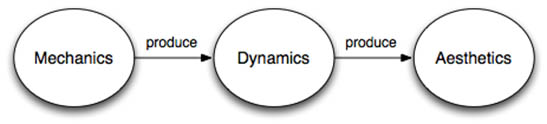
\includegraphics[width=8cm]{assets/mda.jpg}
    \caption{MDA framework\protect\footnotemark}
    \label{fig:mda}
\end{figure}
\footnotetext{\url{http://www.firstpersonscholar.com/a-working-theory-of-game-design}, Accessed: 02-03-2018}

As MDA splits games into three components they can be used as views on different layers of games.
These views enable looking at games from both a designer's perspective but also from the player's perspective.
Players naturally view games from the opposite direction: Aesthetics define the experience, which are created by observable dynamics, which in turn are the result of mechanics.
The following sections discuss the components of MDA starting from a player's perspective which is in line with experience-driven design \cite{Hunicke2004}.

\subsection{Aesthetics}
The authors defined a taxonomy of eight elements to describe the aesthetics of a game: (1) Sensation (sense-pleasure), (2) fantasy (make-believe), (3) narrative (drama), (4) challenge (obstacle course), (5) fellowship (social framework), (6) discovery (uncharted territory), (7) expression (self-discovery), and (8) submission (pastime).
This taxonomy aims to extend the previously limited vocabulary with meaningful categories.
Games are certainly not limited to only one or a subset of these aesthetics.
Instead they tend to emphasize each aesthetic to a different degree.

\subsection{Dynamics}
Dynamics are responsible for producing different aesthetic experiences.
It is useful for designers to understand which types of dynamics influence various aesthetics areas.
As an example (4) challenge can be induced by limiting time, placing obstacles and letting the player face opponents.
Conceptualizing models of gameplay dynamics provides insights into their behavior and potentially highlights deficiencies.
This is especially useful for probabilities as common misconceptions might lead sub-optimal experiences.

\subsection{Mechanics}
Mechanics span the player's affordances (actions, controls) as well as the game space itself (worlds, objects, characters).
The sum of basic mechanics supports the dynamics during gameplay.
This is commonly visible as emergent behavior in games where players attempt to fool their opponents or use specific strategies to their own advantage.
Carefully modifying the underlying mechanics of a game allows designers to influence the resulting dynamics.
The ``Mario Kart'' series by Nintendo is a prominent example featuring mechanics initially designed to help players on lower ranks to overtake their opponents more easily.
Players are able to collect items throughout the course; their strength and overall usefulness greatly depends on the current rank of a player.
However, most of the time this item distribution results in an undesired dynamic during gameplay.
As players in the back are rewarded with powerful, chaotic items they tend to entangle their nearby opponents in ongoing fights.
Meanwhile, players at the top of the ranking enjoy relatively weak attacks and can defend their position more easily.